\section{Background}\label{sec:background}




\begin{figure}[tbp]
    \centering
    \begin{minipage}[t]{0.48\columnwidth}
        \centering
        \includegraphics[height=0.5\columnwidth,trim={0.2cm 0 0 0.2cm},clip]{figures/qubit_mapping.pdf}
        \caption{\small Mapping/routing to resolve physical-qubit topology constraints via $ \SWAP $ insertion.}
        \label{fig:qubit_mapping}
    \end{minipage}
    \hfill
    \begin{minipage}[t]{0.48\columnwidth}
        \centering
        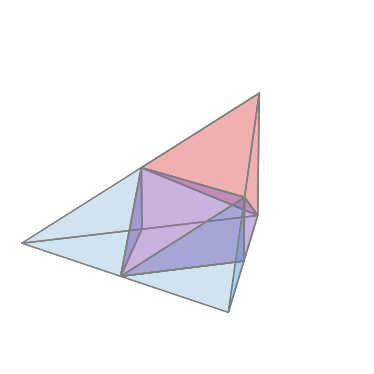
\includegraphics[height=0.5\columnwidth,trim={0.5cm 0.5cm 0.5cm 0.5cm}]{figures/weyl_chamber.pdf}
        \caption{\small Geometric illustration of canonical gates confined to the Weyl chamber.}
        \label{fig:weyl_chamber}
    \end{minipage}
\end{figure}

\footnote{For convenient visualization}


\subsection{Qubit mapping/routing}

Qubit placement and routing ... for connectivity-limited devices


\subsection{Quantum gates realization in diverse ISAs}



\begin{definition}[Canonical gate]
    Any 2Q gate $ U \in \mathbf{SU}(4)$ can be expressed by the composition of its unique \emph{canonical} form
    \begin{align}
        \Can(a,b,c) := e^{-i \frac{\pi}{2}(a\, XX + b\, YY + c\, ZZ)},\, \frac{1}{2} \geq a \geq b \geq \lvert c \rvert
        % U = (A_0\otimes A_1) \Can(a,b,c) (B_0\otimes B_1) = (A_0\otimes A_1) e^{-i \frac{\pi}{2}(a\, XX + b\, YY + c\, ZZ)} (B_0\otimes B_1)
    \end{align}
    sandwiched by local 1Q gates such that we call \emph{$ U $ is locally equivalent to the canonical form $ \Can(a,b,c) $}. %  $ U = (A_0\otimes A_1) \Can(a,b,c) (B_0\otimes B_1) $.
\end{definition}


Canonical representation is ubiquitous as an effective ... 

\ZY{It is ubiquitously used in many quantum computing task ...}




Although there are other conventions .... 
This definition aligns with the \code{TK2} operation definition in \tket, ...



\Cref{fig:weyl_chamber} .....



\begin{align}
    \pSWAP(\theta) \sim \Can(\frac{1}{2},\frac{1}{2},\frac{1}{2}-\frac{\theta}{\pi})
\end{align}



\begin{align}
    \XX(\theta) = \Can(\frac{\theta}{\pi},0,0) \sim \YY(\theta) \sim \ZZ(\theta)
\end{align}
